% vim: set tw=78 tabstop=4 shiftwidth=4 aw ai:
\documentclass{beamer}

\usepackage[utf8x]{inputenc}		% diacritice
\usepackage[english]{babel}
\usepackage{color}			% highlight
\usepackage{alltt}			% highlight

% highlight; comment this out in case you don't input code source files
\usepackage{code/highlight}		% highlight

\usepackage{hyperref}			% folosiți \url{http://...}
					% sau \href{http://...}{Nume Link}
\usepackage{verbatim}

\mode<presentation>
{ \usetheme{Berlin} }

% Încărcăm simbolurilor Unicode românești în titlu și primele pagini
\PreloadUnicodePage{200}

% Arătăm numărul frame-ului
\newcommand{\frameofframes}{/}
\newcommand{\setframeofframes}[1]{\renewcommand{\frameofframes}{#1}}

\setframeofframes{of}
\makeatletter
\setbeamertemplate{footline}
  {%
    \begin{beamercolorbox}[colsep=1.5pt]{upper separation line foot}
    \end{beamercolorbox}
    \begin{beamercolorbox}[ht=2.5ex,dp=1.125ex,%
      leftskip=.3cm,rightskip=.3cm plus1fil]{author in head/foot}%
      \leavevmode{\usebeamerfont{author in head/foot}\insertshortauthor}%
      \hfill%
      {\usebeamerfont{institute in head/foot}\usebeamercolor[fg]{institute in head/foot}\insertshortinstitute}%
    \end{beamercolorbox}%
    \begin{beamercolorbox}[ht=2.5ex,dp=1.125ex,%
      leftskip=.3cm,rightskip=.3cm plus1fil]{title in head/foot}%
      {\usebeamerfont{title in head/foot}\insertshorttitle}%
      \hfill%
      {\usebeamerfont{frame number}\usebeamercolor[fg]{frame number}\insertframenumber~\frameofframes~\inserttotalframenumber}
    \end{beamercolorbox}%
    \begin{beamercolorbox}[colsep=1.5pt]{lower separation line foot}
    \end{beamercolorbox}
  }
\makeatother

\setbeamertemplate{navigation symbols}{}%remove navigation symbols

\title[Improving OpenVPN Performance Using Multipath Link
Aggregation]{Improving OpenVPN Performance Using Multipath Link Aggregation}
\subtitle{Master Report Session -- June 2014}
\institute{Faculty of Automatic Control and Computers,\\
	University POLITEHNICA of Bucharest}
\author[Silviu Petria, Silviu-Mihai Popescu]{Silviu Petria, Silviu-Mihai
Popescu\\
	Supervisor: Costin Raiciu}
\date{June 11, 2014}

\begin{document}

% Slide-urile cu mai multe părți sunt marcate cu textul (cont.)
\setbeamertemplate{frametitle continuation}[from second]

\frame{\titlepage}

\section{Context}
\begin{frame}{Context}
  \begin{itemize}
    \item OpenVPN
    \begin{itemize}
      \item secure point-to-point communication
      \item overhead due to user-space processing
    \end{itemize}
    \item MPTCP
    \begin{itemize}
      \item uses all available links for greater throughput
      \item features like encryption are not part of the design
    \end{itemize}
    \item best of both worlds
  \end{itemize}
\end{frame}

\section{Tuning Linux Networking}
\begin{frame}{Core}
  \begin{itemize}
    \item buffer sizes
    \item inet peer storage
    \item route cache
  \end{itemize}
\end{frame}

\begin{frame}{UDP and TCP}
  \begin{itemize}
    \item buffer sizes
    \item UDP: minimum, pressure, maximum
    \item TCP: minimum, default, maximum
  \end{itemize}
\end{frame}

\begin{frame}{OpenVPN}
  \begin{itemize}
    \item buffer sizes (again)
    \item queue length
    \item tunnel MTU, fragmentation, MSS
    \item no encryption, no HMAC
  \end{itemize}
\end{frame}

\section{Results}
\begin{frame}{Testbed}
  \begin{figure}
    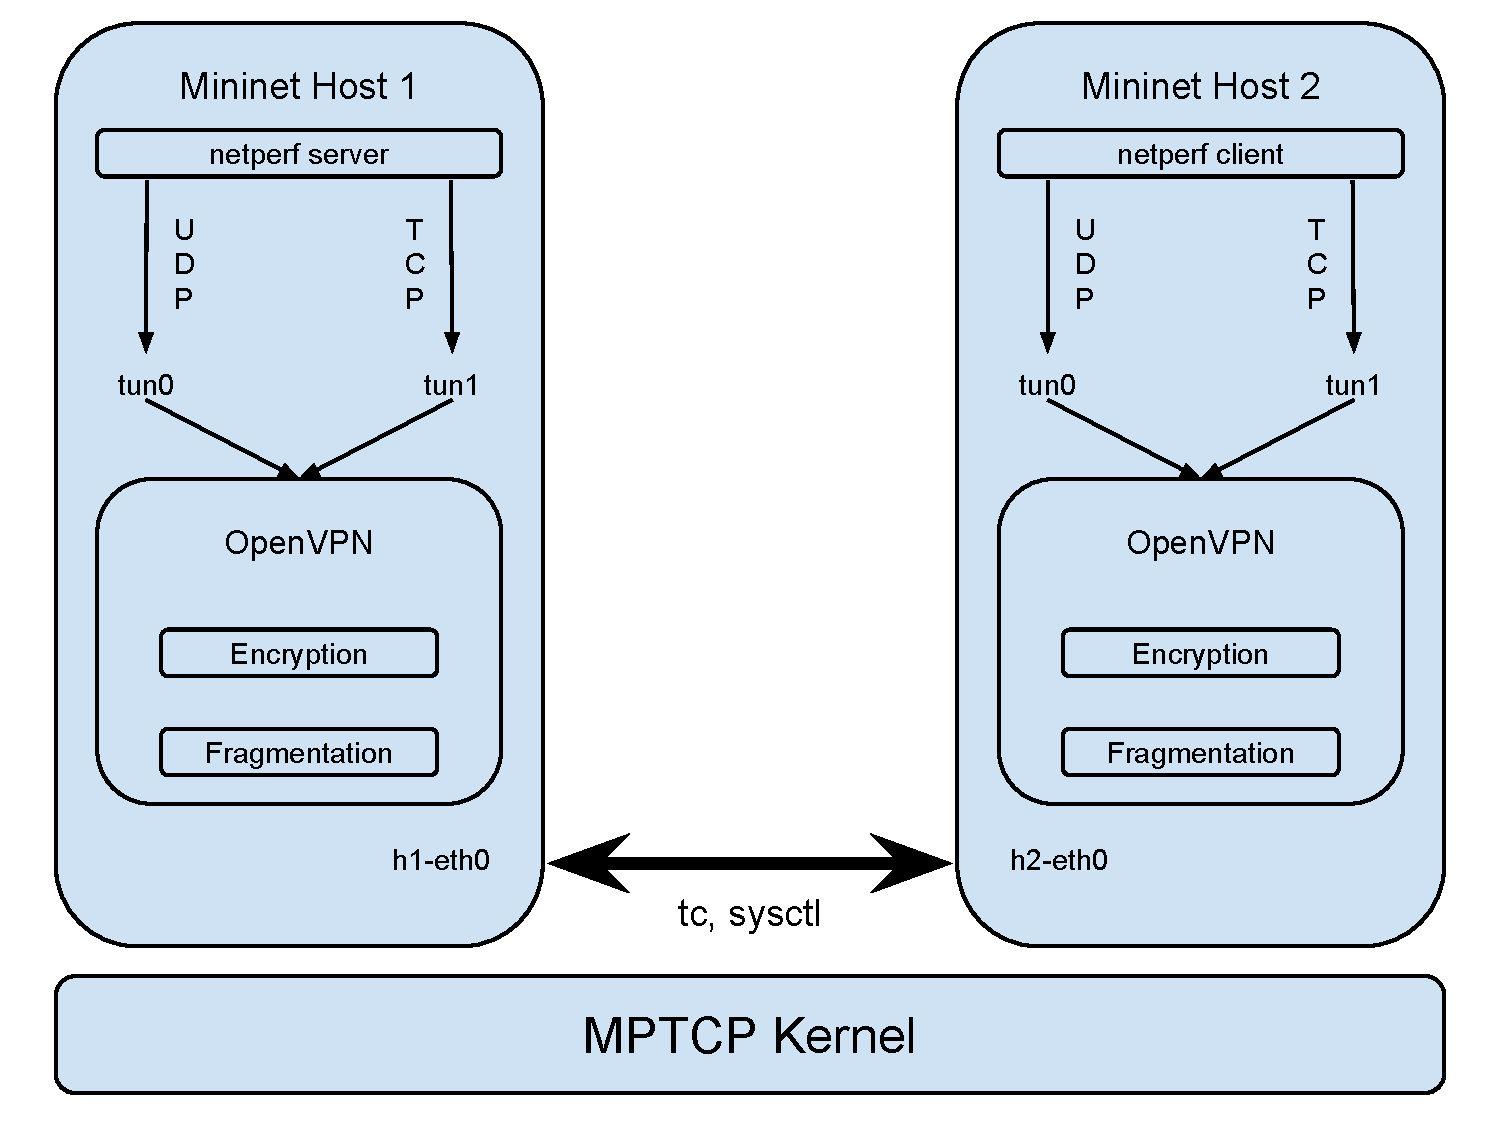
\includegraphics[scale=0.37]{img/mptcp-openvpn}
  \end{figure}
\end{frame}

\begin{frame}{Single UDP tunnel}
  \begin{figure}
    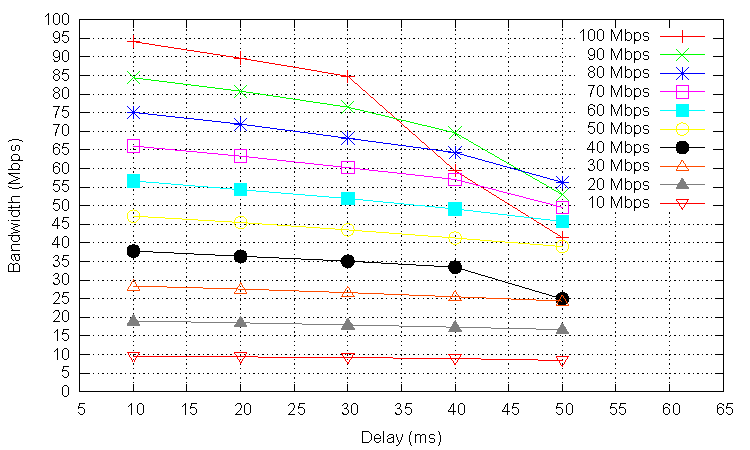
\includegraphics[scale=0.9]{img/test-udp}
  \end{figure}
\end{frame}

\begin{frame}{Single TCP tunnel}
  \begin{figure}
    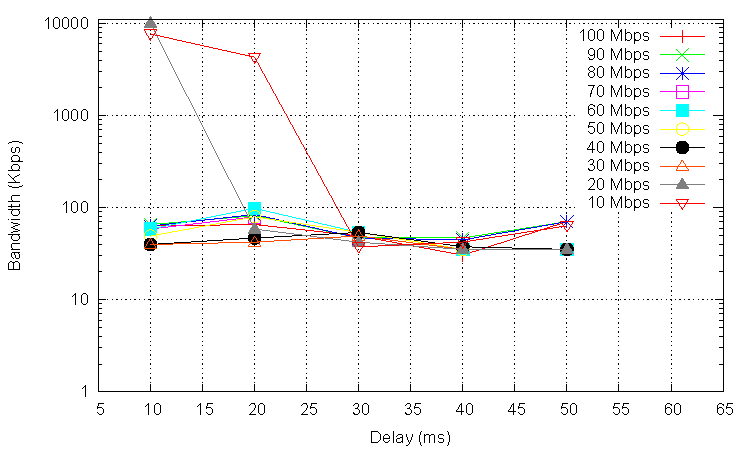
\includegraphics[scale=0.9]{img/test-tcp}
  \end{figure}
\end{frame}

\begin{frame}{UDP and TCP tunnels}
  \begin{figure}
    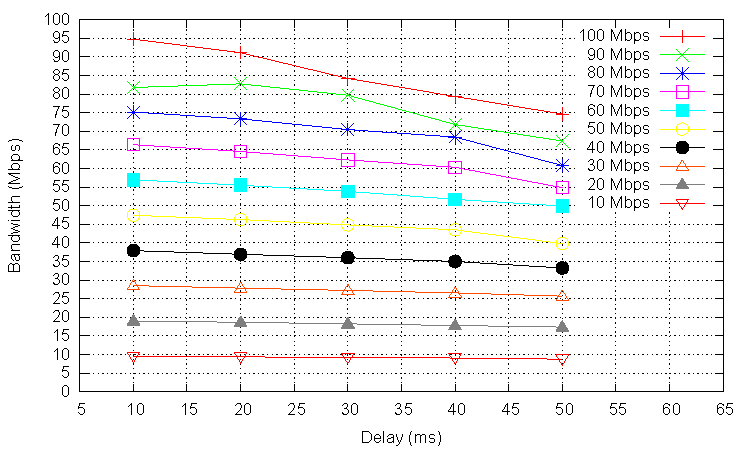
\includegraphics[scale=0.9]{img/test-mptcp-2}
  \end{figure}
\end{frame}

\begin{frame}{UDP and TCP tunnels, default encryption settings}
  \begin{figure}
    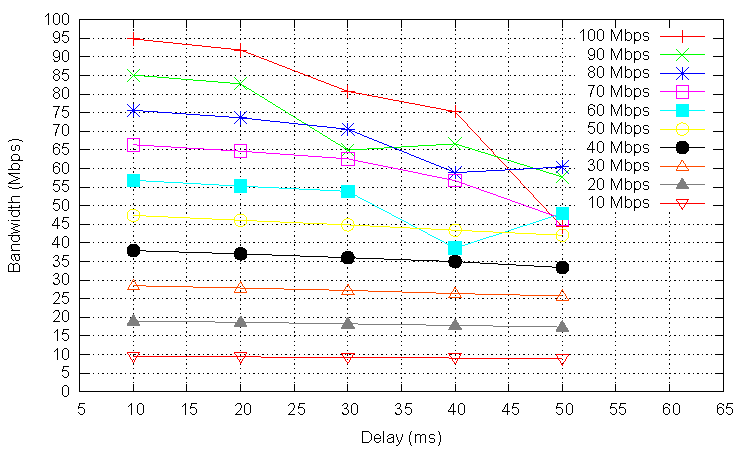
\includegraphics[scale=0.9]{img/test-mptcp-2-crypto}
  \end{figure}

\end{frame}

\section{Conclusions}
\begin{frame}{Conclusions and Further Work}
\begin{itemize}
    \item MPTCP is able to move traffic depending on congestion
    \item best results achieved when socket buffer is twice the BDP
    \item reduce amount of virtualization
    \item dynamically create tunnels based on available protocols
  \end{itemize}
\end{frame}

\end{document}
